\documentclass[a4paper,oneside,DIV=12,12pt]{scrartcl}

%%% Length calculations
\usepackage{calc}
%%%

%%% Support for color
\usepackage{xcolor}
\definecolor{lightblue}{HTML}{03A9F4}
\definecolor{red}{HTML}{F44336}
%%%

%%% Graphics inclusion
\usepackage{graphicx}
%%%

%%% Font selection
\usepackage{fontspec}

\setromanfont{STIX Two Text}[
]

\setsansfont{Source Sans Pro}[
]

\setmonofont{Source Code Pro}[
]

\usepackage{unicode-math}
\setmathfont{STIX Two Math}

%%%

%%% Font settings for different KOMA Script elements
\setkomafont{pagenumber}{\rmfamily}
\setkomafont{disposition}{\rmfamily\bfseries}
%%%

%%% Typographic enhancements
\usepackage{microtype}
%%%

%%% Language-specific settings
\usepackage{polyglossia}
\setmainlanguage{ukrainian}
%%%

%%% List settings
\usepackage{enumitem}
\setlist[enumerate]{
	leftmargin = *,
}
%%%

%%% Captions
\usepackage{caption}
\usepackage{subcaption}

\DeclareCaptionLabelFormat{closing}{#2)}
\captionsetup[subtable]{labelformat = closing}
%%%

%%% Tables
\usepackage{booktabs}
\usepackage{longtable}

\usepackage{multirow}

\usepackage{array}
\newcolumntype{v}[1]{>{\raggedright\arraybackslash\hspace{0pt}}p{#1}}
\newcolumntype{b}[1]{>{\centering\arraybackslash\hspace{0pt}}p{#1}}
\newcolumntype{n}[1]{>{\raggedleft\arraybackslash\hspace{0pt}}p{#1}}
%%%

%%% Links and hyperreferences
\usepackage{hyperref}
\hypersetup{
	colorlinks      = false,
	linkbordercolor = red,
	urlbordercolor  = lightblue,
	pdfborderstyle  = {/S/U/W 1.5},
}
%%%

%%% All caps
\newcommand{\allcaps}[1]{{\addfontfeatures{LetterSpace = 3}#1}}
%%%


\begin{document}
	\begin{titlepage}
	\centering
		Міністерство освіти і науки України\\
		Національний авіаційний університет\\
		Навчально-науковий інститут комп'ютерних інформаційних технологій\\
		Кафедра комп'ютеризованих систем управління

		\vspace*{\fill}

		Лабораторна робота №1\\
		з дисципліни «Архітектура комп'ютерів»\\
		на тему «Синтез керуючих автоматів по графу мікропрограми»\\
		Варіант №4

		\vspace*{\fill}
		
		\begin{flushright}
			Виконав:\\
			студент ННІКІТ СП-225\\
			Клокун В.\,Д.\\
			Перевірив:\\
			Зіньков Ю.\,Г.
		\end{flushright}

		Київ 2018
    \end{titlepage}
	
	\section{Мета роботи}
		Закріплення теоретичних знань по синтезу керуючих автоматів із жорсткою логікою.
		
	\section{Хід роботи}
		Згідно з номером варіанта був заданий граф мікропрограми (табл.~\ref{subfig:01-01-mp-graph}). Дані с заданого графа були підготовані для обробки (табл.~\ref{subfig:01-02-array-m}, табл.~\ref{tab:ristpic-conditional-vertices}) та введені у програму \allcaps{РІСТПІК}. Після обробки даних програмою отримали результати: матрицю переходів (рис.~\ref{fig:ristpic-jump-matrix}), структурну таблицю переходів (рис.~\ref{fig:ristpic-structured-jump-table}), вектор розмітки (рис.~\ref{fig:markup-vector}) та кодування станів (рис.~\ref{fig:coding-result}).
		
		\begin{table}[!htbp]
		\centering
			\begin{subtable}[t]{0.45\textwidth}
			\vspace{0em}
			\centering
				\begin{tabular}{v{3em}n{3em}n{3em}r}
					\toprule
						\multirow{2}{3em}[-0.25em]{№ вер\-ши\-ни} & \multicolumn{2}{c}{Зв'язок з верш.} & Зміст\\
						\cmidrule(lr){2-3}
						& 1 & 2 & \\
					\midrule
						 1 &  0 &  2 & — \\
						 2 &  2 &  3 & $x_9$ \\
						 3 &  0 &  4 & $y_1, y_5, y_7$ \\
						 4 &  5 &  6 & $x_1$ \\
						 5 &  0 &  7 & $y_1, y_5, y_{17}$ \\
						 6 &  8 &  7 & $x_2$ \\
						 7 &  0 & 17 & $y_3, y_4$ \\
						 8 &  9 & 12 & $x_3$ \\
						 9 &  0 & 10 & $y_2, y_4$ \\
						10 & 11 & 19 & $x_4$ \\
						11 &  0 & 12 & $y_6, y_{10}, y_{18}$ \\
						12 &  6 & 13 & $x_5$ \\
						13 &  0 & 14 & $y_1, y_7, y_8$ \\
						14 & 18 & 15 & $x_6$ \\
						15 &  0 & 16 & $y_9, y_{10}$ \\
						16 &  0 & 20 & $y_{12}, y_{15}, y_{16}$ \\
						17 & 10 & 19 & $x_7$ \\
						18 &  0 & 11 & $y_{13}, y_{14}$ \\
						19 &  0 &  5 & $y_7$ \\
						20 & 21 &  1 & $x_8$ \\
						21 &  0 &  6 & $y_{11}, y_{14}$ \\
					\bottomrule
				\end{tabular}
				\subcaption{}
				\label{subfig:01-01-mp-graph}
			\end{subtable}
			\quad
			\begin{subtable}[t]{0.45\textwidth}
			\vspace{0em}
			\centering
				\begin{tabular}{v{3em}n{3em}n{3em}}
					\toprule
						\multirow{2}{3em}[-0.25em]{№ вер\-ши\-ни} & \multicolumn{2}{c}{Зв'язок з верш.}\\
						\cmidrule(lr){2-3}
						& 1 & 2 \\
					\midrule
						 1 &  0 &  2\\
						 2 &  2 &  3\\
						 3 &  0 &  4\\
						 4 &  5 &  6\\
						 5 &  0 &  7\\
						 6 &  8 &  7\\
						 7 &  0 & 17\\
						 8 &  9 & 12\\
						 9 &  0 & 10\\
						10 & 11 & 19\\
						11 &  0 & 12\\
						12 &  6 & 13\\
						13 &  0 & 14\\
						14 & 18 & 15\\
						15 &  0 & 16\\
						16 &  0 & 20\\
						17 & 10 & 19\\
						18 &  0 & 11\\
						19 &  0 &  5\\
						20 & 21 &  1\\
						21 &  0 &  6\\
					\bottomrule
				\end{tabular}
				\subcaption{}
				\label{subfig:01-02-array-m}
			\end{subtable}
		\caption{Мікропрограма: \subref{subfig:01-01-mp-graph}~— заданий граф, \subref{subfig:01-02-array-m}~— масив~$M$ для програми \allcaps{РІСТПІК}}
		\label{tab:01-microprog}%
		\end{table}
		
		\begin{figure}
		\centering
			\begin{subfigure}[t]{0.5\linewidth-0.8em}
			\centering
				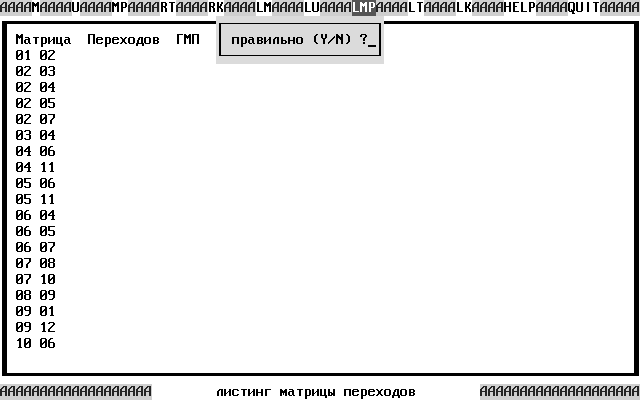
\includegraphics[width = \linewidth]{./assets/00-ris-rus_000-bw.png}
			\end{subfigure}
			\quad
			\begin{subfigure}[t]{0.5\linewidth-0.8em}
			\centering
				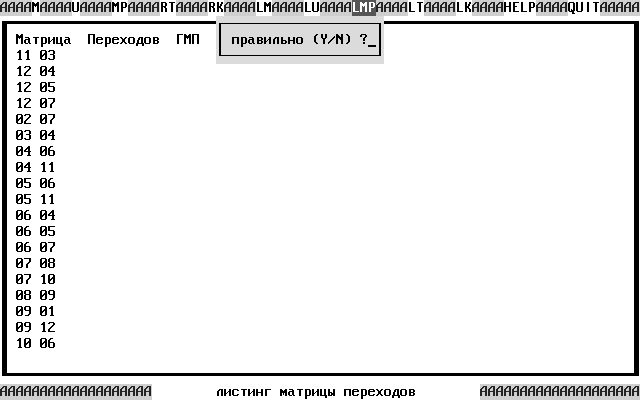
\includegraphics[width = \linewidth]{./assets/01-ris-rus_001-bw.png}
			\end{subfigure}
		\caption{Матриця переходів, згенерована \allcaps{РІСТПІК}}
		\label{fig:ristpic-jump-matrix}
		\end{figure}
		
		\begin{figure}
		\centering
			\begin{subfigure}[t]{0.5\linewidth-0.8em}
			\centering
				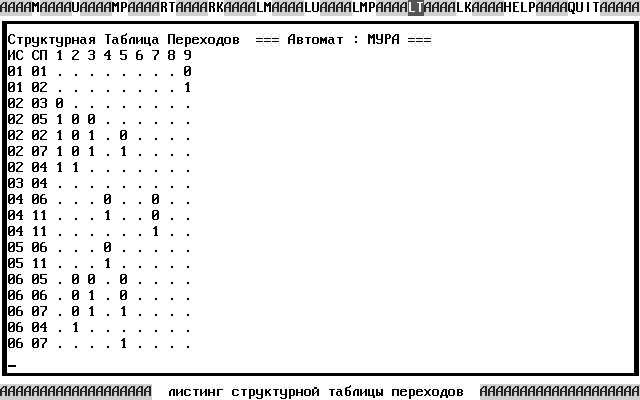
\includegraphics[width = \linewidth]{./assets/02-ris-rus_002-bw.png}
			\end{subfigure}
			\quad
			\begin{subfigure}[t]{0.5\linewidth-0.8em}
			\centering
				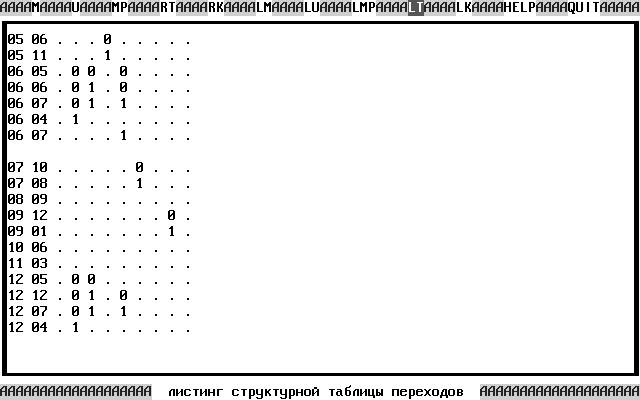
\includegraphics[width = \linewidth]{./assets/03-ris-rus_003-bw.png}
			\end{subfigure}
		\caption{Структурна таблиця переходів, згенерована \allcaps{РІСТПІК}}
		\label{fig:ristpic-structured-jump-table}
		\end{figure}
		
		\begin{figure}
		\centering
			\begin{minipage}{0.5\linewidth-0.8em}
			\centering
				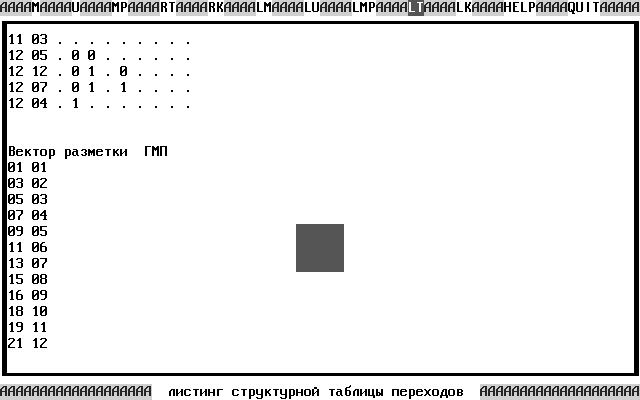
\includegraphics[width = \linewidth]{./assets/04-ris-rus_004-bw.png}
				\captionof{figure}{Вектор розмітки}
				\label{fig:markup-vector}
			\end{minipage}%
			\quad
			\begin{minipage}{0.5\linewidth-0.8em}
			\centering
				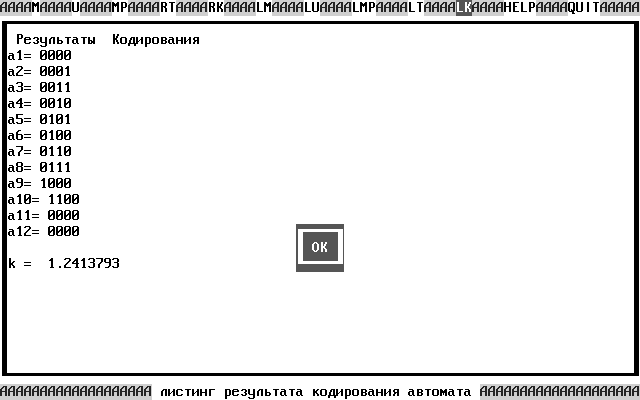
\includegraphics[width = \linewidth]{./assets/05-ris-rus_005-bw.png}
				\captionof{figure}{Результат кодування автомата}
				\label{fig:coding-result}
			\end{minipage}
		\end{figure}
		
		\begin{longtable}{lrn{4em}}
			\toprule
				№ & Вершина & Вхідний сигнал\\
			\midrule
			\endhead
			\bottomrule
			\caption{Масив~$U$ (умовні вершини)}
			\endfoot
			\label{tab:ristpic-conditional-vertices}%
				1 &  2 & 9\\
				2 &  4 & 1\\
				3 &  6 & 2\\
				4 &  8 & 3\\
				5 & 10 & 4\\
				6 & 12 & 5\\
				7 & 14 & 6\\
				8 & 17 & 7\\
				9 & 20 & 8\\
		\end{longtable}
	
	% \section{Контрольні питання}
		% \subsection{Яке призначення керуючих автоматів?}
		% \subsection{У чому складається відмінність автоматів Мілі й Мура?}
		% \subsection{У чому полягає канонічний метод синтезу керуючих автоматів?}
		% \subsection{Назвіть основні етапи структурного синтезу керуючих автоматів за графом мікропрограми.}
		% \subsection{Намалюйте структурну схему керуючого автомата.}
		% \subsection{Для чого необхідно оптимальне кодування станів автомата?}
	
	\section{Висновок}
		Під час виконання даної лабораторної роботи ми закріпили теоретичні знання з синтезу керуючих автоматів із жорсткою логікою.
\end{document}